\documentclass[10pt]{scrreprt}
\usepackage[a4paper, top=30mm, left=30mm, right=20mm, bottom=30mm]{geometry}
\usepackage[utf8]{inputenc}

%Options: Sonny, Lenny, Glenn, Conny, Rejne, Bjarne, Bjornstrup
\usepackage[Bjornstrup]{fncychap}
\usepackage{ngerman}
\usepackage{graphicx}
\usepackage{etoolbox}
\usepackage{enumitem}
\usepackage{numprint}

\makeatletter
\patchcmd{\@makechapterhead}{\vspace*{50\p@}}{\vspace*{-20\p@}}{}{}
\patchcmd{\@makeschapterhead}{\vspace*{50\p@}}{\vspace*{-20\p@}}{}{}
\makeatother


\begin{document}

\thispagestyle{empty}
\title{Pflichtenheft}

\begin{figure}
	\begin{flushright}
		
\includegraphics[scale=0.4]{uniLogo.eps}
		\vspace{2.0 cm}
	\end{flushright}
\end{figure}
\begin{center}
\vspace{2.0 cm}
{\LARGE SEP – Wintersemester 2013/14}

\vspace{1.0 cm}
\textbf{{\Huge Pflichtenheft}}

\vspace{0.8 cm}
\begin{figure}[!htb]
\begin{center}
	%
\includegraphics[scale=1.0]{projektLogo.eps}
	
\includegraphics[scale=1.5]{Logo-Print.eps}
\end{center}
\end{figure}

\vspace{0.2 cm}
\textbf{{\Huge OpenStreetMap: Die Welt in 3D}}

\vspace{1.5 cm}
[endgültiges Datum]

\vspace{0.5 cm}
Version: 1.0

\vspace{1.5 cm}
{\Large Projektbetreuer: Peter Barth}

\vspace{1.5 cm}
\begin{tabular}{|c|c|c|}
\hline 
\rule[-1ex]{0pt}{4ex} \textbf{Phase} & \textbf{Verantwortlicher} & \textbf{E-Mail Adresse} \\ 
\hline  \hline
\rule[-1ex]{0pt}{4ex} Pflichtenheft & Gabriele Haas & haasgab@fim.uni-passau.de \\ 
\hline  \hline
\rule[-1ex]{0pt}{4ex} Entwurf & Thomas Eder & ederthom@fim.uni-passau.de \\ 
\hline  \hline
\rule[-1ex]{0pt}{4ex} Spezifikation & Christof Blauberger & blauberg@fim.uni-passau.de \\ 
\hline  \hline
\rule[-1ex]{0pt}{4ex} Implementierung & Fabian Knorr & knorrfab@fim.uni-passau.de \\ 
\hline \hline 
\rule[-1ex]{0pt}{4ex} Testing & Constantin Wenger & ? \\ 
\hline  \hline
\rule[-1ex]{0pt}{4ex} Präsentation & Sebastian Reichl & reichlse@fim.uni-passau.de \\ 
\hline 
\end{tabular}

\end{center}



\tableofcontents



\chapter{Ausgangssituation}
[Wie stellt sich die Situation heute dar?]

Die Kartendaten des OpenStreetMap-Projekts erfreuen sich immer größerer Beliebtheit. Der Detailgrad der Daten, die Menge an verschiedenen Merkmalen und die Genauigkeit der Daten sind in den meisten Regionen der Welt ihrer Konkurrenz weit voraus. Durch die verschiedenartigen Karten, Kartenstile und Spezialanwendungen auf Basis von OpenStreetMap gibt es eine unzählige Menge von Anwendungsmöglichkeiten.


[Was ist der Auslöser für die Erstellung des Pflichtenhefts?]

Aus diesem Grund soll eine 3D-Desktopanwendung basierend auf den Daten von OpenStreetMap erstellt / implementiert werden.




\chapter{Produkteinsatz}
\section{Produktvision}
Das Ziel des Projekts besteht darin, eine Desktopanwendung zu entwickeln, die eine 3D-Ansicht der Welt mit Hilfe freier Daten aus dem OpenStreetMap-Projekt bietet. Die grafische Benutzeroberfläche zeigt dafür eine Weltkugel, die frei gedreht und gezoomt werden kann. 

Als Oberflächentextur kann dafür anfangs auf die freien Satellitenbilder der
NASA zurückgegriffen werden, beim hineinzoomen in die Karte wird dann auf eine Kartenansicht von OpenStreetMap gewechselt.

Die einfach zu bedienende Oberfläche bietet eine simple Steuerung via Maus und Tastatur und erlaubt zudem in verschiedene Einstellungen die Darstellung der Welt zu beeinflussen. 


\section{Anwendungsbereich}


\section{Zielgruppe}
Primäre Zielgruppe des Systems sind Privatpersonen (Jugendliche sowie erwachsene Personen), die eine andere Art der Kartendarstellung als die typischen Onlinekarten bevorzugen.

Eine weitere Zielgruppe sollen wissbegierige Kinder darstellen. Voraussetzung ist lediglich der geübte Umgang mit der Maus und/ oder Tastatur. (Eingeschränkte Features)

\section{Betriebsbedingungen}
Lebensdauer, Ausfallsicherheit, Beaufsichtigung(Wartung)

\begin{itemize}
\item Bestehende dauerhafte Internetverbindung zum Laden des Kartenmaterials.
\item Nach  der  Abschlusspräsentation  werden  von  uns  keine  weiteren 
Veränderungen vorgenommen. Es erfolgt keine Wartung durch uns.
\end{itemize} 

\section{Sicherheit, Datenschutz, gesetzliche Vorgaben}
Verwendung von OpenStreetMap, Jogl usw. ist lizenzfrei...




\chapter{Produktumgebung}
\section{Software}
\begin{itemize}
\item Windows 7, Windows 8, Linux mit Xorg/KDE4 oder Gnome3 oder vergleichbarem Fenstermanager
\item Java7 
\end{itemize}


\section{Hardware}
\begin{itemize}
\item Aktueller internetfähiger Standard PC
\item RAM: mindestens 2GB
\item Grafikkarte: OpenGl Unterstützung
\item Speicherplatz: 
\end{itemize}


\section{Orgware}
\begin{itemize}
\item Internetverbindung: Breitband, mindestens 1MBit/s
\end{itemize}

User: Jugendliche/Erwachsene
User: Kinder
Schnittstellen: Es  werden  diverse  externe  Quellen genutzt, darunter OpenStreetMap Kartenmaterial, die im laufenden Projekt noch konkretisiert werden.




\chapter{Zielbestimmungen}
[WIE soll WAS erreicht werden?]
Aufgabenstellung / Zielsetzung

\section{Musskriterien}
\begin{itemize}
\item Drehen, Kippen, Zoomen
\item Ansicht Kugel / Flach
\item Satellit / OpenStreetMap
\item Overlays Städte / POIs
\item Anzeige Zoomstufen, Maßstab
\item Längen/Breitengradfelder
\item Englisch \& Deutsch
\item Ladenbalken für Kartendaten; Laden im Hintergrund
\item Seitenleiste zum Einklappen
\item Serverauswahl mit Möglichkeit zur Eingabe eigener Server
\item Bedienung mit Maus 
\item Sinnvolle Beschränkung der Zoomstufen und Beweglichkeit 
\item Limit für gleichzeitig geladene Overpass-Einträge
\end{itemize}
\section{Wunschkriterien}
\begin{itemize}
\item Kinderansicht
\item Höhenprofil
\item 3D-Modelle für Häuser/Bäume
\item Sonnensystem-Modellansicht
\item Höhenlinien
\item Sternenhimmel
\item Tag-/Nachtmodus für Karten
\item Punkte Markieren (Stecknadel, mit Notiz)
\item Suchfunktion, Lokal/Global
\item Eingabeprofile (Rechts-/Linkshänder)
\item Alternative Bedienung mit Tastatur
\item Vollbildmodus
\item Touch-Kompatiblität mit Windows 8
\item Nur rendern wenn nötig (Bildänderung)
\item Antialiasing / Anisotropes Filtern
\item Minimal geladene Tiles
\end{itemize}
\section{Abgrenzungskriterien}
\begin{itemize}
\item Keine First-Person-Ansicht
\item Keine Druck / Speicherfunktion für Kartenmaterial
\item Keine Speicherfunktion für markierte Punkte
\item Keine dyn. Flüsse, ...
\item Kein Routenplaner
\item Keine Unterstützung für Eingabegeräte wie Joysticks
\end{itemize}





\chapter{Produkteinsatz}
\section{Produktvision}
Das Ziel des Projekts besteht darin, eine Desktopanwendung zu entwickeln, die eine 3D-Ansicht der Welt mit Hilfe freier Daten aus dem OpenStreetMap-Projekt bietet. Die grafische Benutzeroberfläche zeigt dafür eine Weltkugel, die frei gedreht und gezoomt werden kann. 

Als Oberflächentextur kann dafür anfangs auf die freien Satellitenbilder der
NASA zurückgegriffen werden, beim hineinzoomen in die Karte wird dann auf eine Kartenansicht von OpenStreetMap gewechselt.

Die einfach zu bedienende Oberfläche bietet eine simple Steuerung via Maus und Tastatur und erlaubt zudem in verschiedene Einstellungen die Darstellung der Welt zu beeinflussen. 


\section{Anwendungsbereich}


\section{Zielgruppe}
Primäre Zielgruppe des Systems sind Privatpersonen (Jugendliche sowie erwachsene Personen), die eine andere Art der Kartendarstellung als die typischen Onlinekarten bevorzugen.

Eine weitere Zielgruppe sollen wissbegierige Kinder darstellen. Voraussetzung ist lediglich der geübte Umgang mit der Maus und/ oder Tastatur. (Eingeschränkte Features)

\section{Betriebsbedingungen}
Lebensdauer, Ausfallsicherheit, Beaufsichtigung(Wartung)

\begin{itemize}
\item Bestehende dauerhafte Internetverbindung zum Laden des Kartenmaterials.
\item Nach  der  Abschlusspräsentation  werden  von  uns  keine  weiteren 
Veränderungen vorgenommen. Es erfolgt keine Wartung durch uns.
\end{itemize} 

\section{Sicherheit, Datenschutz, gesetzliche Vorgaben}
Verwendung von OpenStreetMap, Jogl usw. ist lizenzfrei...




\chapter{Produktfunktionen}

\nplpadding{2}
\renewcommand{\labelenumi}{\textbf{/F\numprint{\theenumi}0/}}

\section{Fensterverhalten}
\begin{enumerate}[leftmargin=2cm]
\item Das Programmfenster startet mit einer Größe von 1024x768 Pixeln. Die Größe ist mit 800x600 Pixeln nach unten, aber nicht nach oben beschränkt und kann vom Benutzer beliebig  verändert werden.
\item Die Anwendung bietet einen Vollbildmodus, in dem Kartenansicht mit Seitenleiste über den gesamten Bildschirm gestreckt werden und Fensterdekorationen entfallen. Zwischen Fenster- und Vollbildmodus kann mit dem Tastenkürzel F11 gewechselt werden.
\item Mit dem Tastenkürzel Strg+Q wird die Anwendung ohne Rückfrage beendet.
\end{enumerate}
\section{Kartenansicht}
\begin{enumerate}[leftmargin=2cm,resume]
\item Die Kartenansicht kann interaktiv mit Maus oder Tastatur bedient werden.
\item Im Sonnensystemmodus 
\item Im 2D-Kartenmodus kann die Ansicht nach links/rechts und oben/unten verschoben sowie (perspektivisch) gekippt werden. 
\item Im 3D-Kartenmodus kann die Ansicht kann um die Erdachse sowie in Richtung der Pole gedreht; ab einem gewissen Zoomlevel am Kameraursprung gekippt werden.
\item Mit Linksklick-Ziehen oder den Pfeiltasten der Tastatur wird die Karte verschoben bzw. der Globus gedreht, mit Rechsklick-Ziehen nach oben/unten oder den BildAuf/BildAb-Tasten der Tastatur wird die Ansicht gekippt.
\item Mit einem einfachen Linksklick werden im Detailfenster zusätzliche Daten zum Punkt unter dem Mauszeiger angezeigt. Bei POIs sind das Adresse sowie Beschreibung; bei anderen Punkten genauer Längen- und Breitengrad.
\end{enumerate}
\section{Navigationsdaten}
\begin{enumerate}[leftmargin=2cm,resume]
\item Das Zoomlevel kann über einen Schieber angezeigt und geändert werden.
\item Der Längen- und Breitengrad des Punktes an der Bildschirmmitte wird über Eingabefelder angezeigt, und kann über sie geändert werden.
\item Ein Ladebalken zeigt den Fortschritt eventuell im Hintergrund geladener Kartendaten an.
\item Der Maßstab des Punktes unter dem Anzeigemittelpunkt wird in einem Feld angezeigt.
\end{enumerate}

\section{Ansichtseinstellungen}
\begin{enumerate}[leftmargin=2cm,resume]
\item Es kann zwischen 3D- (Globus) und 2D-Ansicht (Aufsicht) gewählt werden.
\item Es besteht eine Auswahl aus verschiedenen Kartentypen; wie Satellitenbildern und Straßenkarten.
\item Wird als Kartentyp die Kinder-Weltkarte gewählt, wir eine Auswahl an angezeigten POIs vorgegeben.
\item Es sind Höhenprofile, -linien, sowie 3D-Ansichten von Häusern und Bäumen zuschaltbar.
\item Es können unter einer Vielzahl an Overlays gewählt werden.
\end{enumerate}

\section{Bedienungseinstellungen}
\begin{enumerate}[leftmargin=2cm,resume]
\item Für Linkshänder können die Bedeutungen von linker und rechter Maustaste für die Kartenansicht vertauscht werden.
\end{enumerate}

\section{Detailfenster}
\begin{enumerate}[leftmargin=2cm,resume]
\item Details
\end{enumerate}




\chapter{Produktdaten}

\renewcommand{\labelenumi}{\textbf{/D\numprint{\theenumi}0/}}

\section{Kartenansicht}
\begin{enumerate}[leftmargin=2cm]
\item Verfügbare Kartentypen sind:
\begin{itemize}
\item Satellitenbild
\item OpenStreetMap - Straßenkarte (Tag)
\item OpenStreetMap - Straßenkarte (Nacht)
\item Kinder - Weltkarte
\end{itemize}
\item Wählbare Overlays sind:
\begin{itemize}
\item Städte- und Ländernamen
\item Points of Interest, wie Banken, Tankstellen, Tierparks, Spielplätze etc.
\item Straßennamen
\item Länder- und Staatsgrenzen
\end{itemize}
\end{enumerate}
\section{Kartendaten}
\begin{enumerate}[leftmargin=2cm,resume]
\item Heruntergeladene Kacheln werden primär im Arbeitsspeicher \textbf{(W)} und sekundär in einem Cache im temporären Verzeichnis des Betriebssystems zwischengespeichert.
\item Die Größe der Caches ist einstellbar. Standardmäßig ist der Cache im Arbeitsspeicher 50 MB, der im Dateisystem 200 MB groß.
\end{enumerate}




\chapter{Produktleistungen}

\renewcommand{\labelenumi}{\textbf{/L\numprint{\theenumi}0/}}

\section{Darstellung der Kartenansicht}
\begin{enumerate}[leftmargin=2cm]
\item Aus der aktuellen Perspektive werden die sichtbaren Kartenabschnitte und die nötige Kartenauflösung bestimmt.
\item Das Kartenmaterial ist in Kacheln aufgeteilt, die als Textur auf den Globus bzw. die Karte gelegt werden. Welche Kacheln geladen werden müssen, wird  aus den sichtbaren Kartenabschnitten und dem momentanen Zoomlevel bestimmt.
\item In 3D-Darstellung kann die Ansicht nicht über die Pole hinweg gedreht werden, sodass die Pole im Fenster immer nach oben oder unten zeigen.
\item Overlays wie Städtenamen oder Symbole für Tankstellen werden als zweidimensionale Objekte an die Stelle der Anzeigefläche projiziert, an der der markierte Punkt auf dem Bildschirm erscheint.
\item Dreidimensionale Objekte wie Häusermodelle, Bäume, oder Stecknadeln zur Markierung von Punkten werden direkt in die Szene eingefügt.
\end{enumerate}

\section{Laden der Kartendaten}
\begin{enumerate}[resume,leftmargin=2cm]
\item Ist die Textur einer Kachel bereits geladen, wird sie direkt zur Anzeige verwendet.
\item Ansonsten wird zuerst versucht sie aus dem Cache im Arbeitsspeicher, dann aus dem Cache im Dateisystem zu laden.
\item Ist sie lokal nicht vorhanden, wird sie über einen passenden Kachelserver nachgeladen und dem Cache hinzugefügt.
\item Ist eine Textur noch nicht geladen oder nicht verfügbar, wird sie zwischenzeitlich durch eine Platzhaltertextur ersetzt.
\item Das Laden von Kacheldaten erfolgt im Hintergrund, während die Ansicht weiter gerendert werden kann.
\item Das Laden von Kacheln geschieht über HTTP.
\end{enumerate}

\section{Qualitätsmerkmale}

\begin{enumerate}[leftmargin=2cm,resume]
\item Kartendaten werden effizient zwischengespeichert, um sowohl unnötiges Nachladen als auch den Speicherverbrauch zu minimieren.
\item Der Energieverbrauch wird durch das vermeiden unnötiger Renderzyklen minimiert.
\item Die Anwendung ist intuitiv mit der Toucheingabe auf Windows 8 bedienbar.
\item Die Grafikeinstellungen lassen sich anpassen, sodass die Leistung auch auf älterer Hardware akzeptabel ist.
\item Hintergrundvorgänge des Programms wie das Nachladen von Kartendaten unterbrechen den Rendervorgang nicht.
\item Schlägt das Laden einer Kachel vom Server oder das Übergeben einer Textur an OpenGL fehl, fährt das Programm ohne Unterbrechung unter Verwendung einer Ersatztextur fort.
\item Die Bewegung der Kamera und das anpassen des Zoomlevels wird derart beschränkt, dass keine Darstellungsfehler wie das Durchdringen der Kartenebene auftreten.
\item Die Menge der Angezeigten Overlays und 3D-Modelle wird beschränkt, sodass die Leistung wie auch die Lesbarkeit von Beschriftungen akzeptabel bleibt.
\end{enumerate}




\chapter{Benutzeroberfläche}

\begin{itemize}
	\item Das Hauptelement der Benutzeroberfläche ist die Karten- oder Globusansicht, die sich im rechten Fensterteil befindet. Der sichtbare Kartenausschnitt kann interaktiv mit Maus oder Tastatur verschoben werden.
	\item Im 2D-Modus zeigt die Ansicht eine Projektion der Karte auf die Ebene, die in der Ansicht nach links/rechts und oben/unten verschoben sowie (perspektivisch) gekippt werden kann.
	\item Im 3D-Modus wird ein Globus gezeigt, auf den das Kartenmaterial projiziert wird. Die Ansicht kann um die Erdachse sowie in Richtung der Pole gedreht; ab einem gewissen Zoomlevel am Kameraursprung gekippt werden.
	\item Am linken Rand des Fensters befindet sich eine Seitenleiste, die sämtliche Steuerungsfunktionen bereitstellt. Sie ist in Tabs unterteilt, mit denen die Funktionen gruppiert werden.
\end{itemize}


\begin{figure}
	\centering
	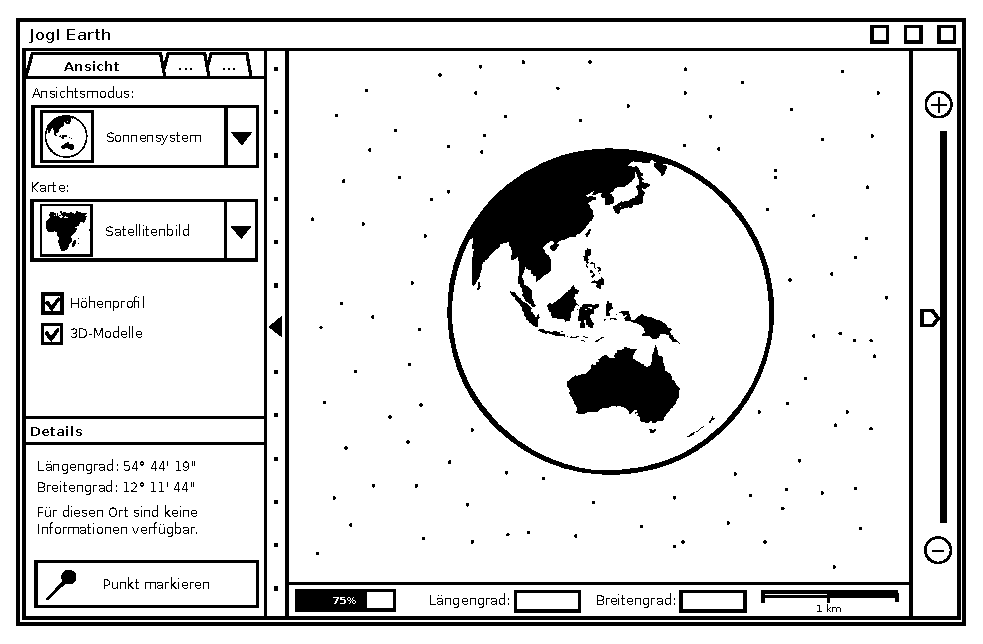
\includegraphics[scale=0.9]{GUI-Ansicht.eps}
	\caption{Die Benutzeroberfläche mit geöffnetem Ansichts-Tab}
\end{figure}
\begin{figure}
	\centering
	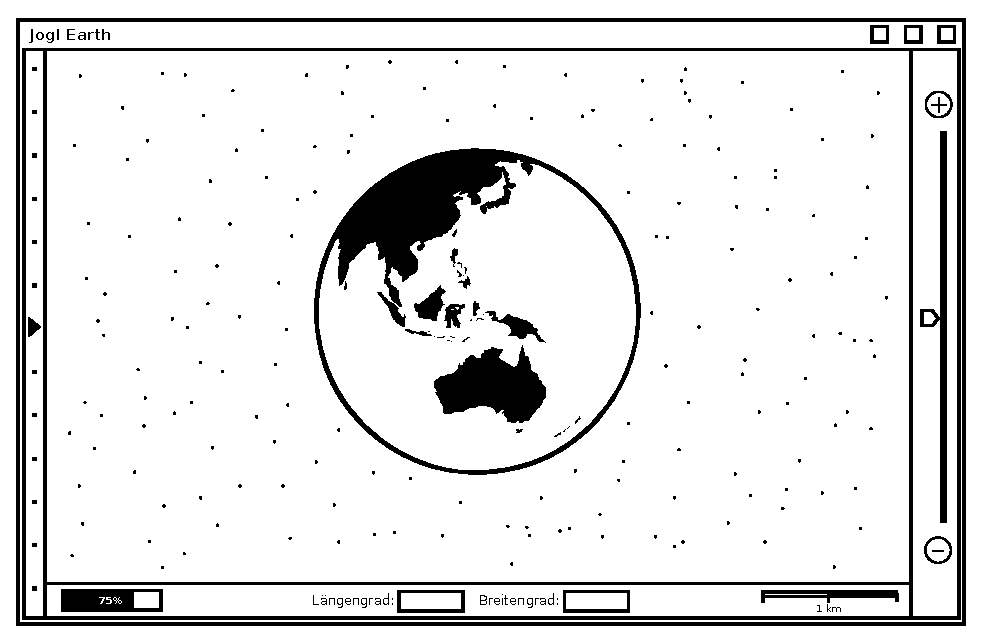
\includegraphics[scale=0.9]{GUI-Ausgeblendet.eps}
	\caption{Die Benutzeroberfläche mit ausgeblendeter Seitenleiste}
\end{figure}
\begin{figure}
	\centering
	\begin{minipage}[c]{6cm}
	\centering
		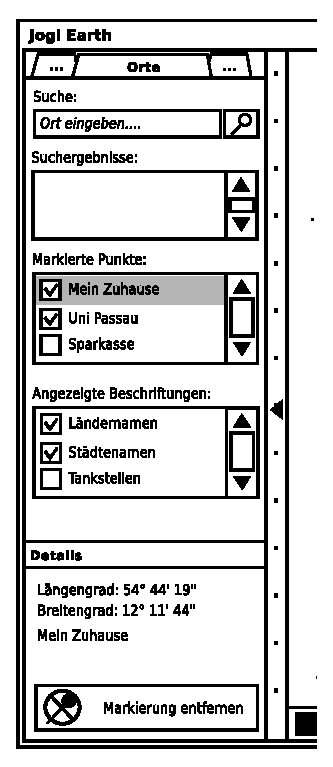
\includegraphics[scale=0.9]{GUI-Orte.eps}
	\end{minipage}
	\begin{minipage}[c]{6cm}
	\centering
		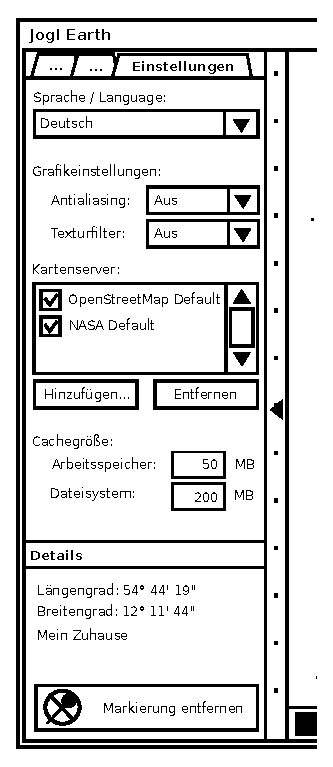
\includegraphics[scale=0.9]{GUI-Einstellungen.eps}
	\end{minipage}
	\caption{Der Orte- und der Einstellungstab}
\end{figure}
\begin{figure}
	\centering
	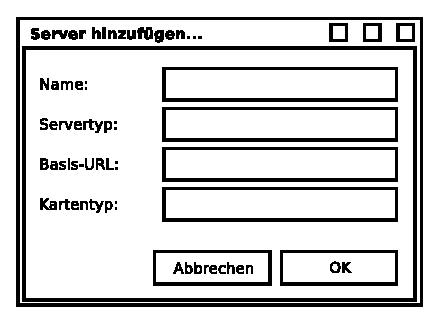
\includegraphics[scale=0.9]{GUI-ServerDialog.eps}
	\caption{Das Dialogfenster zum Hinzufügen eines neuen Servers}
\end{figure}




\chapter{Qualitätsbestimmungen}
\begin{center}
\begin{tabular}{lcccc}
\hline 
\rule[-1ex]{0pt}{4ex} \textit{Produktqualität} & \textit{sehr gut} & \textit{gut} & \textit{normal} & \textit{nicht relevant} \\ 
\hline 
\rule[-1ex]{0pt}{4ex} \textbf{Funktionalität} &  &  &  &  \\ 
\rule[-1ex]{0pt}{4ex} \hspace{10pt} Angemessenheit & • & • & • & • \\ 
\rule[-1ex]{0pt}{4ex} \hspace{10pt} Güte Web-Mining & • & • & • & • \\ 
\rule[-1ex]{0pt}{4ex} \hspace{10pt} Interoperabilität & • & • & • & • \\ 
\rule[-1ex]{0pt}{4ex} \hspace{10pt} Ordnungsmäßigkeit & • & • & • & • \\ 
\rule[-1ex]{0pt}{4ex} \hspace{10pt} Richtigkeit & • & • & • & • \\ 
\rule[-1ex]{0pt}{4ex} \hspace{10pt} Stabilität & • & • & • & • \\ 

\hline 
\rule[-1ex]{0pt}{4ex} \textbf{Zuverlässigkeit} &  &  &  &  \\ 
\rule[-1ex]{0pt}{4ex} \hspace{10pt} Fehlertoleranz & • & • & • & • \\ 
\rule[-1ex]{0pt}{4ex} \hspace{10pt} Wiederherstellbarkeit &  &  &  & • \\ 

\hline 
\rule[-1ex]{0pt}{4ex} \textbf{Benutzbarkeit} &  &  &  &  \\ 
\rule[-1ex]{0pt}{4ex} \hspace{10pt} Bedienbarkeit & • & • & • & • \\ 
\rule[-1ex]{0pt}{4ex} \hspace{10pt} Erlernbarkeit & • & • & • & • \\ 
\rule[-1ex]{0pt}{4ex} \hspace{10pt} Grafische Gestaltung & • & • & • & • \\ 
\rule[-1ex]{0pt}{4ex} \hspace{10pt} Verständlichkeit & • & • & • & • \\ 

\hline 
\rule[-1ex]{0pt}{4ex} \textbf{Effizienz} &  &  &  &  \\ 
\rule[-1ex]{0pt}{4ex} \hspace{10pt} Bildqualität & • & • & • & • \\ 
\rule[-1ex]{0pt}{4ex} \hspace{10pt} Laufzeit & • & • & • & • \\ 
\rule[-1ex]{0pt}{4ex} \hspace{10pt} Speichermanagement & • & • & • & • \\ 

\hline 
\rule[-1ex]{0pt}{4ex} \textbf{Anpassfähigkeit} &  &  &  &  \\ 
\rule[-1ex]{0pt}{4ex} \hspace{10pt} Code-Qualität & • & • & • & • \\ 
\rule[-1ex]{0pt}{4ex} \hspace{10pt} Modifizierbarkeit & • & • & • & • \\ 

\hline 
\rule[-1ex]{0pt}{4ex} \textbf{Portierbarkeit} &  &  &  &  \\ 
\rule[-1ex]{0pt}{4ex} \hspace{10pt} Erweiterbarkeit & • & • & • & • \\ 
\rule[-1ex]{0pt}{4ex} \hspace{10pt} Installierbarkeit & • & • & • & • \\ 
\rule[-1ex]{0pt}{4ex} \hspace{10pt} Konformität & • & • & • & • \\ 

\hline 
\rule[-1ex]{0pt}{4ex} \textbf{Dokumentation} & • & • & • & • \\ 
\hline 
\end{tabular} 
\end{center}




\chapter{Globale Testszenarien und Testfälle}





\chapter{Entwicklungsumgebung}
\section{Software}
\begin{itemize}
\item Windows 7, Windows 8, Linux
\item Eclipse
\item Java 7 (JDK)
\item \LaTeX
\item Git
\item IBM Software Rational Architect
\item ...
\end{itemize}


\section{Hardware}
\begin{itemize}
\item Standard Desktop-PC
\end{itemize}

\section{Orgware}
\begin{itemize}
\item Gruppen-Kommunikation hauptsächlich per Email.
\item Regelmäßige Information des Auftraggebers über die Entwicklungsprozesse/ Phasen/ Ergebnisse.
\end{itemize}




\chapter{Anhang}
\section{Glossar}



\end {document}
